\documentclass[conference]{IEEEtran}
\IEEEoverridecommandlockouts
% The preceding line is only needed to identify funding in the first footnote. If that is unneeded, please comment it out.
\usepackage{cite}
\usepackage{amsmath,amssymb,amsfonts}
\usepackage{algorithmic}
\usepackage{graphicx}
\usepackage{textcomp}
\usepackage{xcolor}
\usepackage{url} 
\def\BibTeX{{\rm B\kern-.05em{\sc i\kern-.025em b}\kern-.08em
    T\kern-.1667em\lower.7ex\hbox{E}\kern-.125emX}}
\begin{document}

\title{CS598 CCC Milestone 2\\
}

\author{
\IEEEauthorblockN{Cameron Greenwalt}
\IEEEauthorblockA{
\textit{UIUC}\\
Champaign, IL, USA \\
cg50@illinois.edu}
\and
\IEEEauthorblockN{Ming Meng}
\IEEEauthorblockA{
\textit{UIUC}\\
Champaign, IL, USA \\
mingm4@illinois.edu}
\and
\IEEEauthorblockN{Yang Peng}
\IEEEauthorblockA{
\textit{UIUC}\\
Champaign, IL, USA \\
yangp3@illinois.edu}
}
\maketitle


\section{Introduction and Project Idea - Edited from Proposal}

AIOps, known as Artificial Intelligence for IT Operations, is a fairly recent development that focuses on applying machine learning to the IT Operations Space. AIOps is a new and exciting area within Cloud Computing and IT Operations. \cite{10212414, 10199929} Many major technology corporations such as IBM and Microsoft \cite{li2022an}  are actively conducting research in the area of AIOps. \cite{aiops-challenges} 

One of the biggest challenges in AIOps is that the cost and time for incorporating AI into the current IT Operations landscape is very expensive. It is often necessary to set-up a team of Machine Learning experts to train the models and understand its workflows. Therefore, we would like to minimize the use of training and finetuning steps by utilizing existing pre-trained Large Language Models (LLM) in the AIOps field.

LLMs have seen tremendous recent breakthroughs, especially in the generative AI space. ChatGPT, which uses OpenAI's GPT 3.5 LLM, was publicly released in late 2022 and had immediate major impacts in many fields. Much research in the industry has been focused on applying LLM and generative chatbots such as ChatGPT to different domains. 

We would like to use generative LLMs to summarize cloud application logs, thereby reducing the effort required for cloud engineers to perform tasks such as system maintenance and problem diagnosis. Existing research on logs in the AIOps space focuses more on log anomaly detection and classification tasks \cite{network-log-anomaly-detection}. Other common AIOps tasks include node failure prediction \cite{aiops-node-failures-alibaba}, CI/CD of ML apps \cite{mlops-ossara}, test case generation and bug detection \cite{model-checking-guided-testing}, task code generation \cite{mani2023enhancing}, incident management \cite{chen2020aiops, li2022an}, and documentation Q\&A/source code understanding \cite{source-code-understanding}. We will focus our research to the task of log summarisation using ChatGPT.


\section{Justification - - Edited from Proposal}
In this section, we present the justifications of the project idea. We believe that this project fulfills all three areas of Intellectual Merit, Novelty, and impact.

\subsection{Intellectual Merit}
Many natural language tasks in AIOps are done using models such as BERT \cite{network-log-anomaly-detection} that are fine-tuned using proprietary data or using rule-based approaches \cite{logrule}. The results with BERT, however, are dismal \cite{network-log-anomaly-detection} in many categories due to issues such as proprietary data availability for training, open source model limitations, and limited hardware acceleration resources. These challenges have hindered some of the development efforts in the AIOps field.

In this project, we will create embedding vectors from log data and use those as a basis of domain-specific knowledge for ChatGPT to tailor its generated log summary output. Prompts will be fed to ChatGPT in Azure cloud, which we believe is a good choice of cloud platform because it has a large market share and is secure.

\subsection{Novelty and Impact}
AIOps has been around for a while. However, as LLM technology is quite new and has only recently gained popularity due to the release of ChatGPT, most AIOps research still revolves around improving existing models/algorithms \cite{network-log-anomaly-detection}. Improving an existing model can be a very expensive operation due to the amount of GPU required for fine-tuning. Many businesses are unable to allocate the resources required to train a model from scratch. The use of traditional ML and DL techniques requires expert domain knowledge and expensive computational resources.

By using pre-trained state-of-art models from existing cloud providers and providing the models domain-specific or proprietary data, one can save computational resources and money by avoiding fine-tuning an existing model or training a model from scratch. This would be a more cost-effective way for businesses' IT teams to roll out AIOps solutions, which will in turn help the business' Site Reliability Engineers (SRE) more effectively address cloud incidents.

If our experiments yield good results, we believe that our work will have a great impact to the AIOps field and that many non-tech companies can apply our methods in small teams of engineers to monitor and improve a company's complex cloud infrastructure environment.

\section{Plan - Edited from Proposal}
We will focus our efforts on the task of cloud log summarisation using generative LLMs.

We have identified some potential areas of difficulty we may encounter in this project:
\begin{itemize}
    \item Dataset selection
    \item Creating embeddings and storing them in Vector stores
    \item Integration with Azure AI Services
    \item Usability
    \item Achieving Good Results
\end{itemize}

For our dataset, we will use a sample set of Proxifier logs from the LogHub \cite{zhu2023loghub}.

We will use ChatGPT to generate our log summaries, as it is better-suited to this task than to other tasks such as anomaly detection and log classification.

\subsection{What system do you want to implement?}
Our system will be known as "A general AIOps framework on log data using LLM-generated results". The system involves a user passing sample log data to our prompt generator application, which will vectorize the provided logs and store them in a vector store. Then, users will submit a natural language query to the chatbot such as "Summarize this log for me: <log>". The chatbot then generates a prompt by utilizing the existing query embeddings from the vector store.

\begin{figure}[ht]
    \centering
    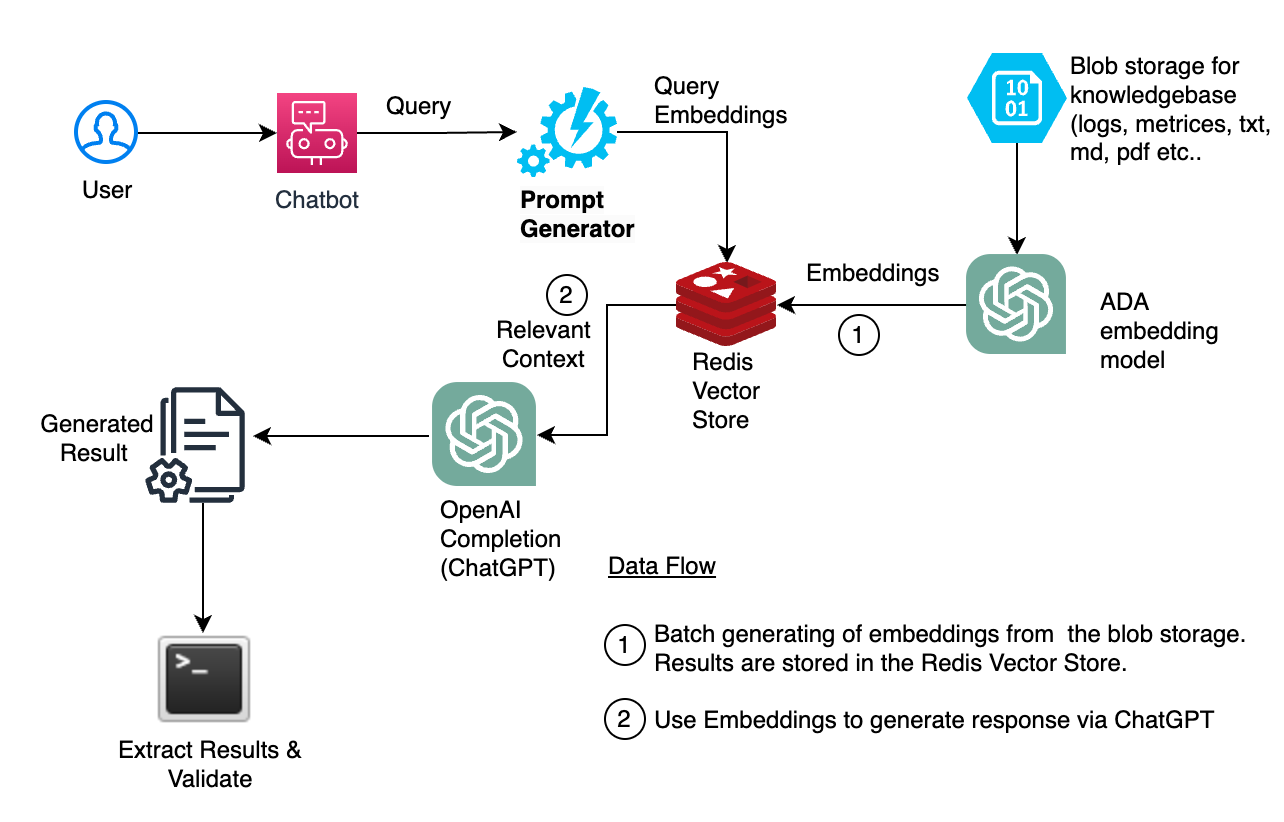
\includegraphics[width=0.4\textwidth]{arch.png}
    \caption{A proposed AIOps framework using LLM-generated results}
    \label{fig:arch}
\end{figure} 

Figure \ref{fig:arch} above shows the proposed implementation of the system. The chatbot can be either UI or API based. We plan to use Redis for the vector store, but another application such as Azure's Cloud AI vector store would work as well. The ADA embedding model will convert the provided data source into vector embeddings, which will be then be stored in the vector store. Then, the user submits a natural language prompt to our system. The prompt then becomes the input for ChatGPT. ChatGPT then uses the prompt, the log embeddings vector store, and its pretrained parameters to generate a summary of the log from the prompt. We will validate the generated result against a prelabeled result text file for accuracy. 


\section{THE EXPERIMENT}

We divide our experiment into two categories: functional and infrastructure. The functional part describes how our system is going to function. The infrastructure part describes how we are going to build the system (e.g. steps, tools, and cloud services).

\subsection{System to Build- Functional}

The system we are trying to build is using ChatGPT to summarize server logs from different applications. We believe that this would be very helpful for Site Reliability Engineers(SREs) for their day-to-day job for use-cases such as system maintenance and cloud incident response. By performing log summarisation tasks through the use of LLM, even non-subject-matter-experts can understand log output and therefore better understand software systems.

Furthermore, management could use the system to get a brief summary of the incident by feeding a few observed log lines to the prompt. The generated summary output could be used by the managers to provide better directions to the engineers. Overall, we envision that this system would improve efficiency, troubleshooting, and understanding.

\subsection{System to Build- Infrastructure}

Note that this section contains information from the Figure 1 in our plan above. However, the main components in our system include the following:

\begin{enumerate}
    \item User- The users are mainly SREs or engineers working on incidents. Management could also use this tool to obtain brief summary of an incident.
    \item Chatbot- This is the UI that the user will interact with.
    \item Prompt Generator- This is how the prompt will be generated, from matching the query embeddings stored in the Vector Stores.
    \item Data Source- The data source can be from various log sources within LogHub.
    \item Embedding model- We plan to use ADA embedding model available in Azure Cloud.
    \item Vector Store - Redis or Azure Vector Store
    \item Output validation- Pre-labeled data-set, different metric scores, and/or manual validation.
\end{enumerate}

In regards to our data source, we plan to proceed with utilizing logs from LogHub \cite{zhu2023loghub}, which is a public repository in GitHub and contains a collection of system/application logs that are made freely accessible for AI-driven log analysis. The logs are preproccessed in any way.

For the data selection, we plan to experiment with Proxifier logs, which is a software that performs network proxy tasks. The reasons for starting with Proxifier are that the software is simple and the dataset is small enough for us to perform manual validation. Additionally, the Proxifier website has extensive documentation on how the software works.

\subsection{Hypothesis to Test}\label{AA}

Below we propose 7 hypotheses and experiments to test. These experiments will test our system's ability to generate correct and readable summaries. We willincorporate the use of lexical and semantic scores to compare the relationships of the measurement outcomes.

\subsubsection{should be able to handle text summarization}
\begin{itemize}
    \item \textbf{model}: gpt-4-32k or gpt-35-turbo-16k 
    \item \textbf{input}: sample logs
    \item \textbf{output}: log summarization
    \item \textbf{measurements}:
    \begin{itemize}
        \item correctness
        \item readability
        \item Lexical score if possible
        \item Semantic score if possible
    \end{itemize}
\end{itemize}

\subsubsection{should be able to handle large text(over 100kb)}
\begin{itemize}
    \item \textbf{model}: gpt-4-32k or gpt-35-turbo-16k 
    \item \textbf{input}: sample logs
    \item \textbf{output}: log summarization
    \item \textbf{measurements}:
    \begin{itemize}
        \item correctness
        \item readability
        \item Lexical score if possible
        \item Semantic score if possible
    \end{itemize}
\end{itemize}


\subsubsection{should be able to get lexical score for a given text}
\begin{itemize}
    \item \textbf{input}: log summarization
    \item \textbf{output}: lexical score 
    \item \textbf{measurements}:
    \begin{itemize}
        \item human validation
    \end{itemize}
\end{itemize}

\subsubsection{should be able to get Semantic score for a given text}
\begin{itemize}
    \item \textbf{input}: log summarization
    \item \textbf{output}: Semantic score 
    \item \textbf{measurements}:
    \begin{itemize}
        \item human validation
    \end{itemize}
\end{itemize}

\subsubsection{should be able to create and store the embedding from the input logs}
\begin{itemize}
    \item \textbf{model}: ada
    \item \textbf{input}: sample logs
    \item \textbf{output}: log embedding
    \item \textbf{measurements}:
    \begin{itemize}
        \item searchable by similarity
    \end{itemize}
\end{itemize}

\subsubsection{should be able to store embedding into the vector store}
\begin{itemize}
    \item \textbf{input}: embedding vector
    \item \textbf{output}: vector store
    \item \textbf{measurements}:
    \begin{itemize}
        \item embedding should be persistent
    \end{itemize}
\end{itemize}

\subsubsection{should be able query the embedding from the vector store}
\begin{itemize}
    \item \textbf{input}: embedding input
    \item \textbf{output}: embedding output
    \item \textbf{measurements}:
    \begin{itemize}
        \item embedding should be searchable
    \end{itemize}
\end{itemize}



For the first two experiments, we will select sample logs of a cloud environment for our data source to validate that the generated result of a simple prompt works in terms of correctness and readability. It could be a simple question such as "what does this log-line do". We plan to experiment with multiple lines of logs to validate that our system can handle text larger than 100kb.

Proper embedding is critical to the appropriate functionality of our system, so that means we need to test embedding extensively. Our fourth experiment does so by testing the ADA embedding model and measuring embeddings by similarity. The input logs will be fed into the ADA model and output the log embedding, which will be used as the input for our sixth experiment--store the log embedding into the vector store. The embedding should be persistent in the vector store. We should be able to query the vector store and the embeddings should be easily searchable. These will be tested in our final experiment.


\subsection{Measurements and Evaluation}
We will use the ROUGE family of metrics in evaluating the performance of our log summaries. \cite{lin2004rouge} ROUGE metrics are a standard in the industry for text summarization evaluation. These metrics work by comparing a generated summary to a reference or "gold-standard" summary produced by a human. The dataset we plan to use in our research already includes human-created summaries for each log. We will use these preexisting, human-generated summaries as the standard for computing the ROUGE metrics.

We will also record several metrics relating to the performance of our system in the cloud such as latency of performing requests and running inferences, estimated cost of compute/storage, bandwidth limit, etc.

\subsection{Expected Successful Results}
We will compare the ROUGE F1 scores of our system to that of a very simple, no-ML baseline method \cite{medium-text-summarization} and to that of LogSummary. \cite{10017337}

We will also perform qualitative analysis on our log summary. We understand that this step is subjective and may not come with a discrete metric, but we feel that human evaluation is beneficial in this case. It is important to evaluate the results manually as we need to ensure that the results are readable and make sense to our intended audiences such as SREs, developers, and even their managers.

\section{Literature Surveys}
Below are the literature Surveys we conducted in terms log summerization, AIOps for Logs, and AIOps with Incident Management. We've done a tremonduos amount of reading to arrive refine our project idea and experiments to ensure the novelty and impact of the system which we're trying to build.

\subsection{CAMERON'S LITERATURE SURVEY - Log Summarisation}

LogRule \cite{logrule} is a Root Cause Analysis (RCA) algorithm, which, with a high F1-score of 0.921 and a 37x speed improvement over FP-growth, offers a time-efficient, accurate, and interpretable solution for RCA in complex datasets, especially where the current state-of-the-art algorithm struggles with execution times. LogRule aims to provide an explanation for specific events of interest, but it depends on structured rather than unstructured logs, which means that doing log preprocessing or overhauling a system's logs to all be structured would be prerequisites to using the system.

Auto-logging \cite{10173904} is an idea proposed wherein AI is used to automatically inject structured logging into key parts of the source code to enable easier downstream log analysis methods, possibly using AI. The authors that proposed auto-logging correctly point out two key assumptions of the current logging status quo: 1) that humans are to be the end consumers of logs and 2) that the developers that insert the logs into the software have sufficient understanding of the system. Both assumptions have proven to be violated in various cases, which breaking of assumptions introduces challenges in the area of AIOps. While the idea of auto-logging seeks to address the root problem of the current logging paradigm, our work seeks to use NLP and LLMs to act as human-like consumers of logs and digest the information therein, thereby assisting OCEs/SREs/SMEs in their workflows in the current paradigm of logging.

LogSummary \cite{10017337} is perhaps the work in closest relation to what we would like to accomplish in our reasearch. LogSummary is an automatic and unsupervised log summarization framework that achieves an impressive ROUGE F1 score. The authors, upon finding that no preexisting "gold standard" labelled dataset of logs and their associated summaries, created their own dataset of logs and log summaries. This is what they used to assess the quality of their models. We will use their opensource dataset in our work to assess the quality of our methods.

At the core of LogSummary is the LogIE algorithm, which "performs open information extraction on logs, extracting triples relating entities and arguments through relation or predicate." \cite{10017337} LogSummary does \textit{not} use generative LLMs such as ChatGPT. We plan to use LLMs to accomplish a similar objective while not being constrained to a entities-events-relation triples for log summaries as is done in the LogSummary work.

CloudRCA is "a root cause analysis framework for Alibaba Cloud's big data cloud computing platforms, utilizing heterogeneous multi-source data, state-of-the-art anomaly detection, and log analysis techniques to extract features, which are then employed in a Knowledge-informed Hierarchical Bayesian Network (KHBN) model." \cite{10.1145/3459637.3481903} CloudRCA is a thorough, useful system that is in-use in Alibaba's cloud systems and has provided a 20\% time savings for SREs. The cost for an organization to implement CloudRCA or a similar system in their own cloud platforms may exceed its relative benefit, and CloudRCA may not be applicable to somewhat dissimilar use cases. We envision that our work will have more general applicability and lower cost-to-implement for various organizations at the expense of narrower scope of operations (only log summarization).

One area that we may find challenging in our research is in the log preprocessing step of the ML pipeline. We would like our propsed system to generalize to various log sources, but logs have a very diverse set of formatting rules. We may want to consider parsing/preprocessing logs using methods and software proposed by the authors in \cite{10.1145/3540250.3558947}.

\subsection{JASON'S LITERATURE SURVEY - AIops with Logs}
Presently, lots of AIOps tasks use logs as one of the main data sources. Lots of the research papers focus on log anomaly detection and classification tasks, as they are often achievable through fine-tuning an existing model with a few-shot. 

Based on multiple research papers, it appears that BERT is a very popular model that is used for log anomaly detection. The results are quite successful for very specific tasks such as detection and classification, but it also means that the usage is limited to specific scope with lesser impacts. In addition, the BERT base model requires further training and fine-tuning which can be time-consuming and expensive. \cite{LEE2023110689}

The anomaly log detection task is proved to be very successful in recent research extending the BERT model with fine-tuning. For a sample HDFS data-sets, the F1 score can achieve more than 0.9 in many scenarios. This can attribute to the reason that HDFS log data consists of a very simple log structure and has less natural language included in the logs. In fact, the authors identified that pre-training BERT further with more natural language data had a negative effect on anomaly detection. \cite{LEE2023110689} From the lesson, we identified that LLM is probably more suited for logs with more context of natural language. Therefore, in order to best use of ChatGPT's capabilities, we need to ensure that the logs we chose should contain some natural language texts.

Other current researches on utilizing BERT model for AIOps tasks include using it to build an intelligent-based system for IT Incident Operations. However, the metric scores are quite low with just the base BERT models and often require other classifier such as LSTM which are used for remembering the previous steps to increase accuracy. But this might run into over-fitting issues, a classical ML problem as when using LSTM it tends to remember the information for long-term. \cite{10189040}

As logs from different applications and systems can be in various formatting, it is important that we have to ingest and parse the logs to the intended formatting for our destination. This means data transformation capabilities are required for the data injectors. Current popular open-source tool that are used to ingest data includes Logstash and is currently compliant with multiple databases and agents like Telegraf. Alternatively, many proprietary software may have its own data transformation capabilities that can be used to avoid having an additional third-party dependency. \cite{bendimerad2023onpremise}

Log data can be beneficial for incident management and resolution tasks when we also have past incident data attached with it. Automation can be performed with efficient ML models to generate diagnosis and resolution steps. This is especially powerful for some urgent cases where the assigned engineer can start diagnosing the issue and perform the generated steps for resolution. However, performing this step requires past incident data which are often proprietary and can be difficult to obtain with the existing publicly available resources online, especially we have to find the incident data that contains the logs. \cite{bendimerad2023onpremise}

Generating summaries from log data has also been discussed as future possible research. LLM is very useful in this aspect and can be used especially for this kind of application. Some authors acknowledge that the ChatGPT model is more accurate than many other open source models that are presently available for summary generation and it does not require further training on its own. In the near future, open-source LLM may progress further which can also be used to train and deployed on-premise. But presently the ChatGPT model is used as a golden benchmark for most generative AI tasks.\cite{bendimerad2023onpremise}

Presently, server logs are also used to determine the frequency of page access, access and browsing patterns, and is a field of web mining development. Within the web mining field, the server logs is used in all aspects on the Cloud applications, including e-commerce, corporate email servers, and web reports. It provides information to improve the businesses or systems in terms of user experience and can also be used for providing revenue forecasts. \cite{9898279}

Note that logs alone may not offer enough insights. Technical documentations, knowledge articles, and/or past incident investigations data are also good companions to derive summary or root cause. Some of the data points which are often used with logs include a company's internal root cause knowledge source database, technical documentation on the application or systems, troubleshooting guides, or even the history of bug fixes in the release notes. These information are often unstructured but are beneficial for the generation of analysis and summaries. \cite{saha2022mining}

Just right before ChatGPT API was released, the summarizing part for an AI generated incident analysis is often done through a base pre-trained model with further fine-tuning. One of the popular models that's used is RoBERTa, which is itself a BERT derivative and the authors further fine-tuned on other external or internal datasets, often borrowing popular new websites and articles. \cite{saha2022mining}

Logs are often in semi-structured and in some cases even in unstructured formatting. There are no golden standard for logging specifications and even leading companies like Microsoft and Google had issues with finding a systematic way to guide its developers to agree on a single logging practice. Therefore, challenges arise on log parsing and that the traditional way is to rely on regular expressions, keywords, grammar, algorithms, or even statistics to parse and read the logs. \cite{survey-log-aiops}

One of the current popular ways of parsing logs is through some sort of Clustering, Pattern Mining, and tree-based algorithms. LogMine and LogMa are two popular log parses which uses the idea of clustering with either a K-means algorithm or a hierarchical clustering algorithm. SLCT and LogCluster looks for frequent log file items and perform some kind of frequent pattern mining. \cite{survey-log-aiops}

Applying language model to log parsing and mining is still a quite new and most of the recent researches come from Pre-ChatGPT times. One of the research known as Logram uses traditional NLP methods such as leveraging n-gram dictionaries to achieve such tasks. \cite{10189040}

Prompt generation is often an issue with ChatGPT as an incorrect prompt could lead to incorrect answers. The prompt needs to be carefully constructed and tuned to generate a specific prompt. Embeddings needs to be used as Example selection during the inference phase so that when the user issues a sample input, the system would match the existing embeddings and automatically draft a prompt with relevant information to feed into ChatGPT. Note that logs can belong to non-text input and can exceed the input limit for a lot of LLMs and this needs to be considered. For example, ChatGPT 3.5 has a 3000 words input limitations. \cite{zhoudb}

Overall, the applications of LLM is relatively new within the field of AIOps. There are even authors acknowledging that their future research direction is to incorporate the use of LLM such as ChatGPT into their existing AIOps research. \cite{bendimerad2023premise} We believe that it is the perfect time for us to do so and incorporate this new AI Generation wave within AIOps with the focus of log analysis and log summary.

\subsection{MAX'S LITERATURE SURVEY - AIops with Incident Management}

LLMs. Prompt-engineering research has surged recently, and is necessary to utilize LLMs to their full potential. Some approaches attempt to improve the reasoning quality of LLMs through chain-of-though and scratch-padding, some aim to keep the LLM self-consistent, some use debating among multiple models to improve results, some verify the response. Some approaches provide general-purpose techniques that teach LLMs to use tools, some retrieve useful text from a large corpus and put in context when needed, whilst others provide a systematic architecture for tools to use LLMs. Prior work processes multi-modal data (e.g., image, audio, text, etc.) with LLMs without explicit training\cite{hamadanian2023a} 

Recent advances large language models like GPT-3/4, which have been used to solve a variety of problems ranging from question answering to text summarization. 

some study explored how to generating a chain of thought---a series of intermediate reasoning steps---significantly improves the ability of large language models to perform complex reasoning\cite{wei2022chain}

Some studies demonstrates that in order to improve task-agnostic, few-shot performance, scaling up the language models are often necessary. The GPT-3, which itself is a scaled up model compared to many other language models, can achieve strong performance on many datasets. The NLP tasks that it can achieve include translation and question-answering. \cite{brown2020language}

LLM also widely adopted to use for programming task like Codex. It is actually fine-tuned through publicly available code from GitHub and uses GPT as a base language model.
It is used to generate Python code. \cite{chen2021evaluating}

LLMs can be trained with public and proprietary log data. LLMs can offer an efficient aqnd effective solution for many AIOps tasks. The common tasks include automated log analysis which enables SREs to focus on other mission critical tasks.\cite{gupta2023learning}

Large cloud services often have many incidents, which leads to many researches performed in the incident management area within the Systems and Software Engineering communities. There has been several empirical studies on analyzing incidents and outages in production systems which have focused on studying incidents caused by certain type of issues or issues from specific services and systems.\cite{10172904} 

The following two scenarios was studied using LLM \cite{10172904} 

1) Find the Incident's Root Cause. Diagnosing incidents typically requires significant time and communication before engineers can identify the root cause of the incident. Research showed how effective large language models are at suggesting root causes for incidents\cite{10172904} 

2) Suggest the Mitigation Steps for the Incident. After a root cause has been located, engineers take actions to mitigate the problem. research showed effective large language models are at recommending the mitigation steps for incidents\cite{10172904} 

After I researched over 40,000 incidents from 1000+ cloud services with six semantic and lexical metrics at Microsoft.\cite{10172904}  The results shows:
\begin{itemize}
    \item Fine-tuning significantly improves the effectiveness of LLMs for incident data.
    \item GPT-3 and GPT-3.5 models significantly outperform encoder-decoder models in our experiments.
    \item Metrics such as BLEU-4 are useful to measure relative performance of models in different settings. However, manual inspection and validation with experts is needed to assess the actual performance.
\end{itemize}

\section{Summary}

Overall, we believe that our system is going to benefit companies of all sizes and improve their IT Operations workflows in a modern complex cloud infrastructure, as they often are unable to allocate the necessary resources and budget to train and fine-tune large ML models. We expect the following stakeholders to benefit from this project:
\begin{itemize}
    \item Site Reliability Engineers
    \item Platform Engineers 
    \item Management Audience 
    \item Incident Commanders 
\end{itemize}

We expect that SREs and Platform Engineers are the stakeholders that will benefit the most as our framework can used as an assistance tool for SREs when when maintaining cloud systems or responding to cloud incidents. Managers can use this tool to understand the current situation of the infrastructure without knowing many technical details. The incident commander can use this tool to ensure that the analysis is flowing in the right direction. Finally, we believe now is an optimal time to incorporate Generative AI into the corporate world within the IT Operations field. We hope this framework can transform how incident management, alerting, and root cause analysis are performed. 


\bibliographystyle{plain}
\bibliography{ref}
\vspace{12pt}

\end{document}
